\documentclass{article}

\usepackage[utf8]{inputenc}
\usepackage{amsmath}
\usepackage{graphicx}
\usepackage[colorlinks=true, urlcolor=blue, linkcolor=red]{hyperref}
\usepackage{parskip}
\usepackage[font=small,labelfont=bf]{caption} 

\title{Assignment 1}
\author{Ivan Aristy — iae225}
\date{\today}

\begin{document}

\maketitle

\section{Assignment }
\subsection{Designing a Static Visualization}

Your task for this assignment is to design a static visualization that you believe effectively communicates an idea or message about the sunshine data, and provide a written report (no more than 1 page, single spaced, not including images) that details your design. Note that you should include at least one image of your visualization in your report (i.e., when all of the images are excluded from the report, the text does not exceed 1 page). We recommend that you start this assignment by identifying a question about the data that you would like your visualization to answer. Then, you should design a visualization to answer that question, and use that question as the title of your visualization.

You are required to use the given data set, but you are free to transform the data in any way that you wish. That is, you can manipulate the data using transformations such as a log transformation, computing percentages or averages, grouping elements into categories, or removing unnecessary variables. You are also allowed to incorporate additional data from external sources, but if you do so, you need to make a note of it in your submission.

Remember that different visualizations can emphasize different aspects of a data set, so your writeup should include details about which components of the data you intended to communicate. You should also provide comments on which aspects of the data set are obscured by your visualization design.

Your report should explain the rationale behind your design decisions. You should document the visual encodings you used and why they are effective for communicating your intended message. These decisions include things like the choice of visualization type, size, color, scale, and other visual elements (which we will learn more about during Week \#3 and Week \#4 lectures).

\newpage
Note, the text for this document is under a standard word page when excluding the images and pretty formatting. 

\subsection{Intended Visualization \& Question}

\textbf{During which months are cities between the 68 and 80°F range, 
while maximizing for sunshine hours?}

This is the question we aim to answer in this assignment.
The reason for this question is that the 68-80°F range is considered the most comfortable for most people, 
and sunshine during this time will make living there a better experience. 
The audience would be looking for the best cities climate-wise for a vacation, to move to, or maybe a second house.

\subsection{Data Cleaning \& Gathering}

We first need to consider if we have all the elements necessary to answer this question.
In particular, we already have sunshine hours per month, and the particular cities we want to analyze.
However, we do not have the temperature data for each city. Hence, we can retrieve this data from \href{https://www.weather.gov/wrh/Climate}{weather.gov} 

\begin{center}
    \vspace{0.25cm}
    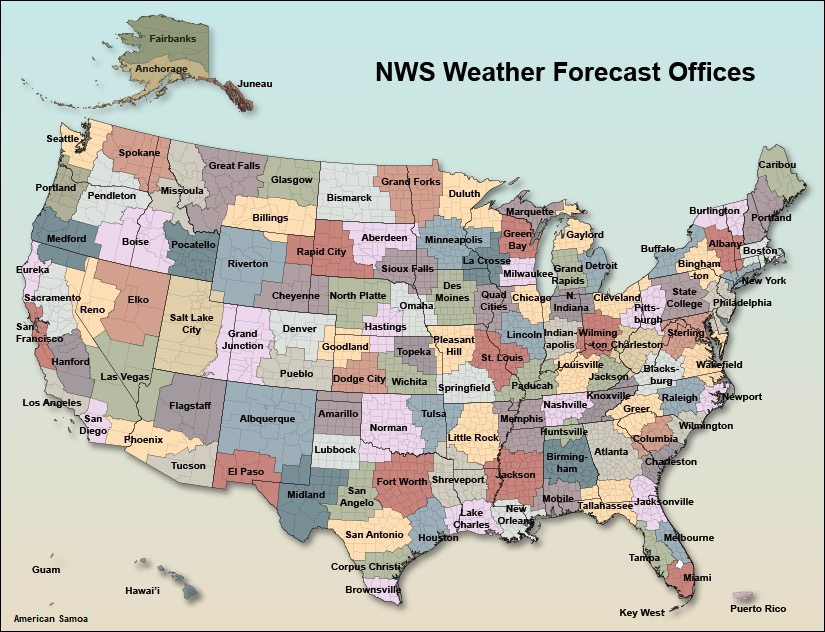
\includegraphics[width=\textwidth]{map.jpg}
    \captionof{figure}{Map of the United States showing available data.}
    
    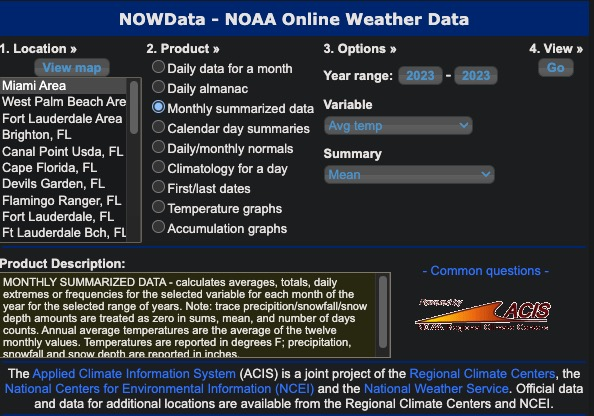
\includegraphics[width=\textwidth]{datarequest.jpg}
    \captionof{figure}{Data request for weather.gov}
    
    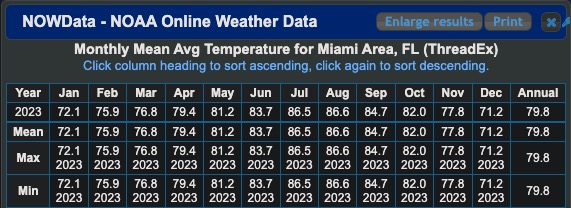
\includegraphics[width=\textwidth]{table.jpg}
    \captionof{figure}{Obtained data for temperature.}
        \vspace{0.5cm}
\end{center}

Also, we do not need to consider latitude and longitude for our visualization, so we can remove or ignorethese columns.

\pagebreak

\subsection{Iterations}
First I tried to filter the data to only show cities with a temperature between 68 and 80°F: 

\begin{center}
    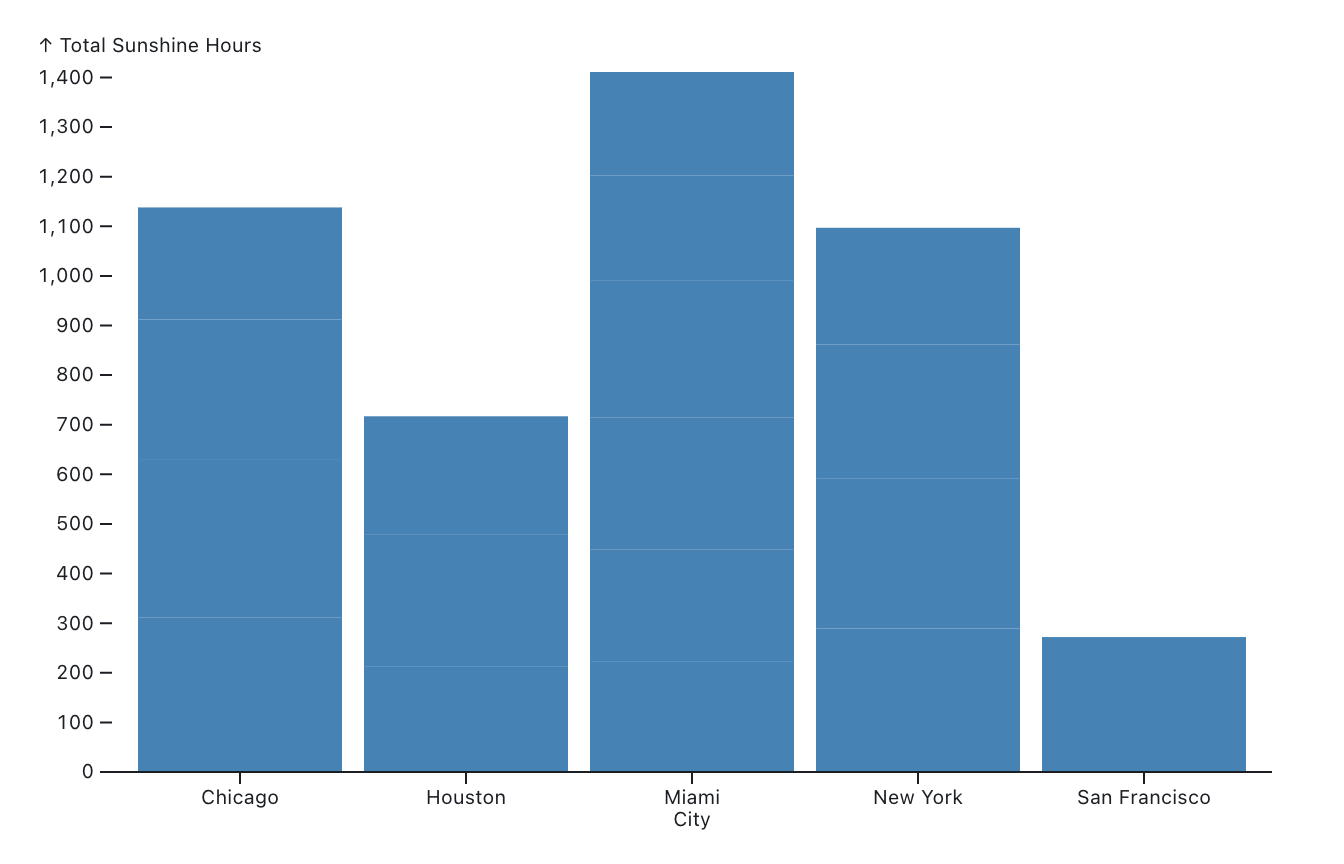
\includegraphics[width=\textwidth]{filter.png}
\end{center}

Ignore, that there's no visual encoding, this is just testing. However, I think this approach is not effective
in communicating the data. We could instead try to encode the data using a scatter plot, with temperature on the x-axis, and sunshine hours on the y-axis.

\begin{center}
    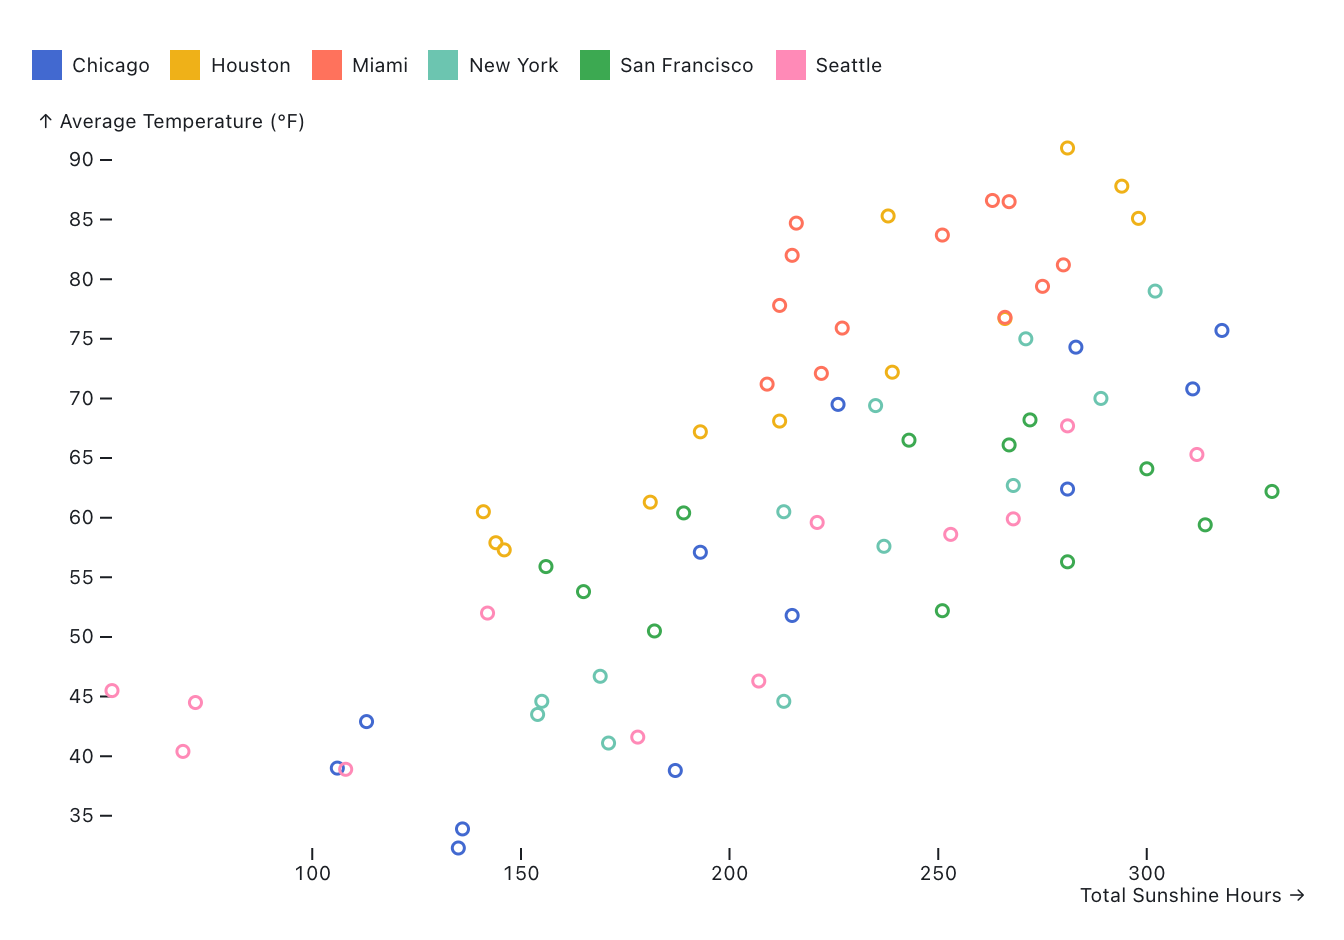
\includegraphics[scale=0.2]{scatter.png}
\end{center}

\pagebreak

Adding a highlighted section for the 68-80°F range:

\begin{center}
    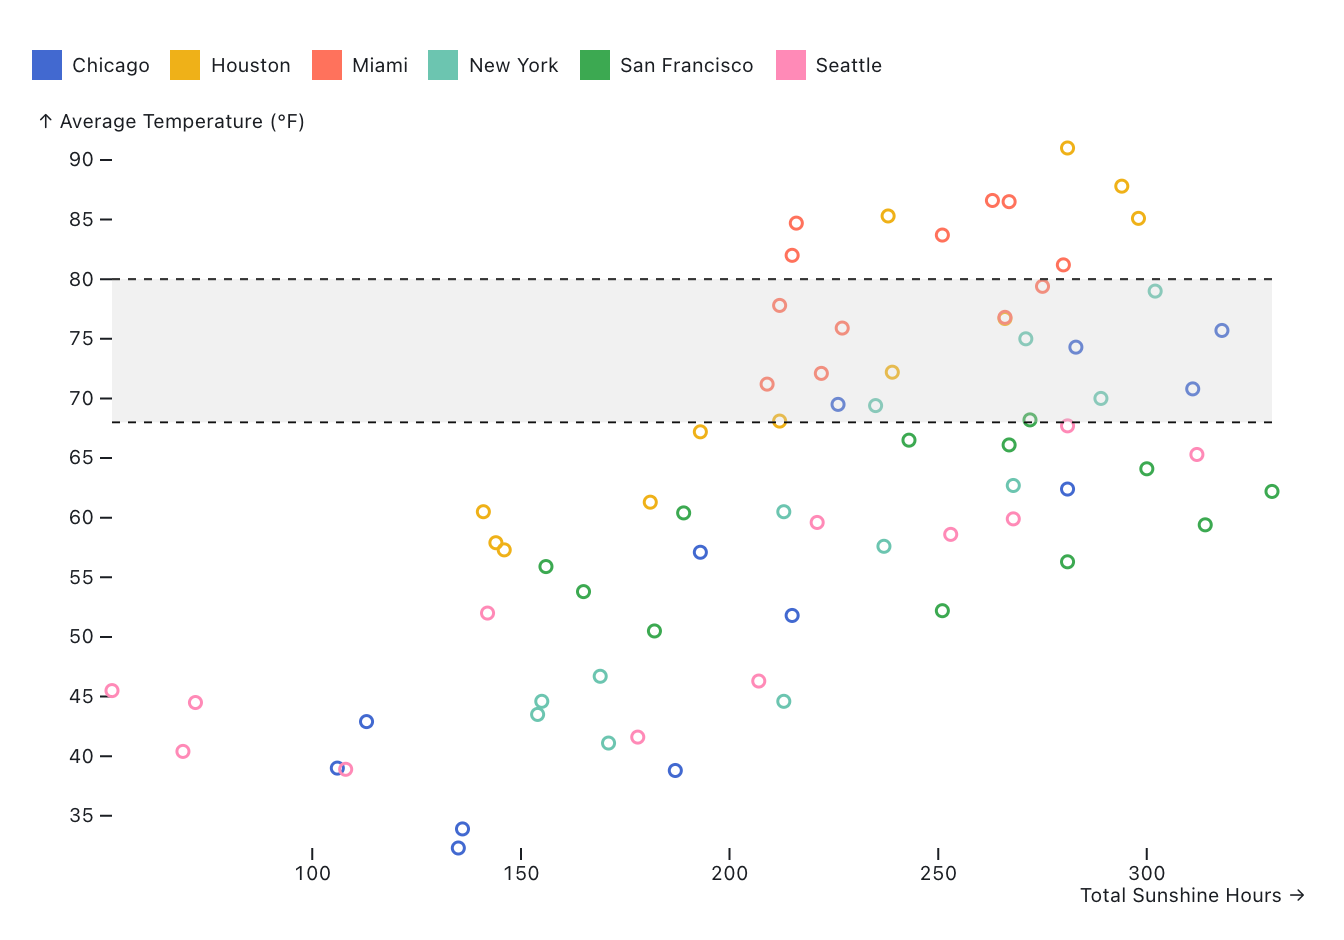
\includegraphics[scale=0.2]{scatter2.png}
\end{center}

This shows more information, but we have (a) non-clarification of months, which is crucial for the audience, and (b) it feels cluttered.

The major issue is that we are trying to represent 4 variables in a 2D space.
I also considered a bubble chart, where the x-axis represents months, 
the y-axis represents the cities, 
the size of each bubble represents sunshine hours, 
and the color of the bubbles represents the temperature.
This would no doubt feel cluttered, and the audience would have a hard time 
interpreting the data.

Hence, the two best approaches are to either filter the data to only 
show cities in the 68-80°F range in a line chart,
or to add two panels for the dependent vars:




\subsection{Final Visualization}
\subsubsection{Does this answer the question?}

\textbf{We highlight some key data:}
\begin{itemize}
    \item \textbf{Sunshine} lorem ipsum dolor sit amet  
    \item \textbf{Temperature} lorem ipsum dolor sit amet
    \item \textbf{City} lorem ipsum dolor sit amet
\end{itemize}

\subsubsection{Encoding (Marks/Channels, Redundancy, Color/Accessibilty)}
\subsubsection{Obscured Data}
    \begin{itemize}
        \item \textbf{Preference:} The visualization is not dynamic, hence we cannot allow the user to select their desired temperature range.
        \item \textbf{Lat-Long:} Our visualization assumes that the audience is familiar with the cities in the dataset, and doesn't provide a map for reference.
        \item \textbf{Humidity:} We do not consider humidity in our visualization, which could be a factor in the comfort of the weather.
    \end{itemize}

\bibliographystyle{plain}
\bibliography{references}

\end{document}